
\section{Efficient implementation}\label{eff_imp}

\begin{figure*}[!t]
\begin{centering}
\begin{tikzpicture}
    \begin{groupplot}
      [group style={%
        columns=2,
        rows=1,
        group name=plots,
        xlabels at=edge bottom,
        %y descriptions at=all,
        horizontal sep=6em,        
      },
      enlarge x limits={abs=.2},
      width=0.48\textwidth,
      height=0.3\textwidth,
      ]
    \nextgroupplot[xlabel=Decomposition rank.,
		ylabel=Residue,
		domain=1:1000]
        \addplot[blue] table {valB_15000.dat};
        \addlegendentry{KPCA}
        \addplot[red] table {valR_15000.dat};
        \addlegendentry{ICD}
        \addplot[green] table {valG_15000.dat};
        \addlegendentry{CCD}
        
    \nextgroupplot[ymode = log,
        xlabel=Decomposition rank.,
		ylabel=Time in s,
		domain=1:1000]
        \addplot[blue] table {lineB_15000.dat};
        \addplot[red] table {lineR_15000.dat};
        \addplot[green, mark=*] coordinates{(14999, 13.2714)};
        
    %\nextgroupplot[xlabel=Decomposition rank,
	%	ylabel=Time in s,
	%	domain=1:1000]
	%	\addplot[blue]\addplot[blue] table {valB.dat};
    %    \addplot[red] table {valR.dat};
    %    \addplot[green] table {valG.dat};
        
    \end{groupplot}    
\end{tikzpicture}
\caption{Comparison between complete Cholesky decomposition (CCD, in green), incomplete Cholesky decomposition (ICD, in red) and kernel PCA (KPCA, in blue), varying the rank of $B$. Left: Residue for each decomposition. Right: Time of calculation. We use SPoC features~\cite{babenko15} of 15000 sample images.}
\label{fig:residue}
\end{centering}
\end{figure*}

When compared to the linear square-loss classifier of Section \ref{slem:intro}, one drawback of the kernelized approach is that the dimension of our problem grows with the size $n$ of the negative samples. The offline factorization $B$ of $K$ demands $O(nr)$ storage and at best $O(nr^2)$ time. 
This factorization can be obtained in two fundamental ways: full-rank and low-rank decomposition. In this section we propose three different decompositions of $K$, to be applied depending on the compromise between accuracy and storage we went to achieve.
%on which of these two efficiencies we hope to achieve.

%As for the online step, solving Equation (\ref{beta:final}) amounts to, for all positive exemplars, calculating the row $[u, v^T]$ of $B'$  from Lemma 1 and solving a linear system in $A$, which is a $(r+1)\times (r+1)$ matrix. The first of these is computed in time $O(nr)$ and the second, $O(r^3)$.

\subsection{Full-rank decomposition}
The complete Cholesky decomposition (CCD) is the most used factorization of positive-definite matrices in kernel-based learning due to its time efficiency \cite{BaJo02}. We use it as our default decomposition.
We make sure $K$ is positive-definite by adding $\epsilon$ to its diagonal, where $\epsilon=\min(0,-\lambda_{min})$ and $\lambda_{min}$ is the smallest eigenvalue of $K$. Therefore, from the equation $BB^T=K+\epsilon\mathrm{Id}_n$, $B$ has rank $n$ and can be calculated by CCD.

\subsection{Low-rank decomposition}
Let us now turn to the problem of improving storage efficiency. One of the major requisites of a global image descriptor for large scale retrieval is to minimize the storage.
As discussed in Section \ref{simi_score}, for each positive exemplar we store its base representation plus a $2r$ vector. Hence, we aim to decompose $K$ at a small rank $r$.
We consider the problem of finding a factor $B$ of fixed rank $r$ such that the residue. We propose two methods of decomposition. $\mathrm{tr}(K-BB^T)/\mathrm{tr}(K)$ is small. \hlc{I wanted to write "factor $B$ of fixed rank $r$ that minimizes the residue $\mathrm{tr}(K-BB^T)/\mathrm{tr}(K)$", but I don't want to propose it as an optimization problem. The "such that the residue is small" is not perfect, but it is the best I could find. Any proposition?}

\textbf{ICD} The incomplete Cholesky decomposition (ICD) is widely used in machine learning~\cite{BaJo02,BaJo05,FiSc01}. Its algorithm is similar to CCD, and it greedily chooses which column of $K$ to add to the decomposition based on the gain in approximation error for all non-added columns. This process is called \emph{pivot selection}~\cite{BaJo05}. We stop the algorithm $r$ steps, obtaining the factor $B$ in time $O(nr^2)$.

\textbf{KPCA} The kernel PCA (KPCA) proposes that, instead of a greedy addition of columns, we choose the $r$ first eigenvectors to form the $r$ columns of $B$. This is done by doing a truncated singular value decomposition of $K$:
\begin{equation}
    K = WDW^T; \ b_i = \sqrt{d_{ii}}w_i, \label{svd}
\end{equation}
where $w_i$ denotes the $i$-th column of $W$ (\ie the $i$-th eigenvector of $K$) and $d_{ii}$ the $i$-th diagonal element of $D$ (\ie the $i$-th eigenvalue of $K$). Decomposing $K$ from Eq.~(\ref{svd}) has complexity $O(n^2r)$ in time.~\cite{golub2012matrix}

We plot in Fig. \ref{fig:residue} the residue $\mathrm{tr}(K-BB^T)/\mathrm{tr}(K)$ when we vary the number of columns $r$ of $B$ and we see a faster convergence for the kernel PCA decomposition when $r$ goes to $n$. Figure \ref{kpca:icd} shows an accuracy comparison between the two decompositions, confirming that KPCA gives a better approximation of the full-rank decomposition.

\begin{figure}[!h]
\centering
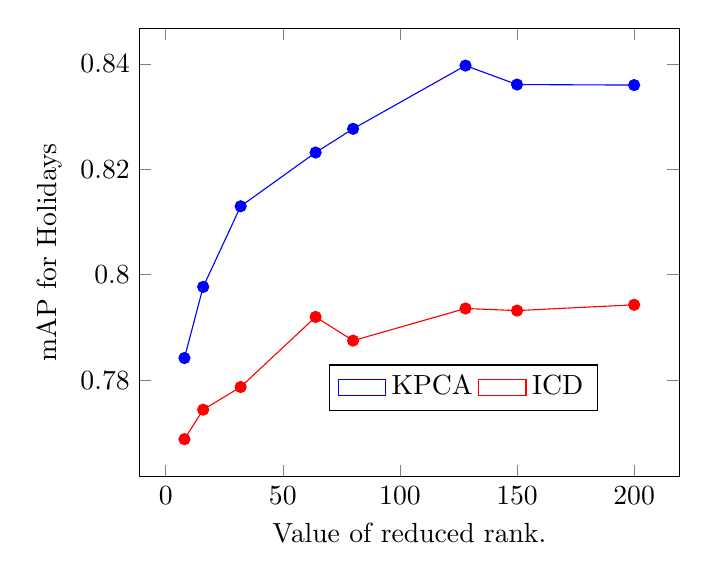
\begin{tikzpicture}
	\begin{axis}[
		xlabel=Value of reduced rank.,
		ylabel=mAP for Holidays,
		legend style={
			area legend,
			at={(0.6,0.25)},
			anchor=north,
			legend columns=-1}]
%%Poly SLEM
    \addplot[mark=*, blue] coordinates{
        (  8, 0.7842)
        ( 16, 0.7977)
        ( 32, 0.8130)
        ( 64, 0.8232)
        ( 80, 0.8277)
        (128, 0.8397)
        (150, 0.8361)
       ( 200, 0.8360)
    };
    \addlegendentry{KPCA}
    \addplot[mark=*, red] coordinates{
        (  8, 0.7688)
        ( 16, 0.7744)
        ( 32, 0.7787)
        ( 64, 0.7920)
        ( 80, 0.7875)
        (128, 0.7936)
        (150, 0.7932)
       ( 200, 0.7943)
    };
    \addlegendentry{ICD}
	\end{axis}
\end{tikzpicture}
\caption{mAP for Holidays using SPoC + Poly SLEM. We perform two low-rank decompositions and compare its results at similar ranks.}
\label{kpca:icd}
\end{figure}



We also compare the time of calculation in Fig. \ref{fig:residue}, which shows that KPCA is slower than ICD for small values of $r$ and faster for values of $r$ such that the residue is small.
\hlc{I could not finish the discussion in this section, I need some sleep...}

%The incomplete Cholesky decomposition (ICD) is the most used factorization of positive-semidefinite matrices in kernel-based learning due to its time efficiency \cite{BaJo02,BaJo05,FiSc01}. The computation of the factor $B$ depends on a permutation $\pi(n) =\{i_1,i_2,\dots,i_n\}$ of $\{1,2,\dots, n\}$, called \textit{pivots}. The $t$-th column of $B$ is calculated iteratively as:

%\begin{align}
%\begin{cases}
%\vspace{3 mm}
%B(i_t, t) = \left(K(i_t,i_t)-\sum_{m=1}^{t-1} B(i_{m},m)  \right)^{\frac{1}{2}},\\
%\vspace{3 mm}
%B(i_j,t) = 0,\\
%B(i_j, t) = \frac{1}{B(i_t,t)}(K(i_j,i_t)  -\sum_{m=1}^{t-1}B(i_j,m)B(i_t,m)), \end{cases}\label{icd:algo}
%\end{align}
%for all $t<j\le n$. 

%There are two possible choices of Cholesky decomposition. The incomplete Cholesky decomposition (ICD) stops its algorithm after $r$ steps and has complexity $O(nr^2)$. 
%To minimize the residue $\mathrm{tr}(K-BB^T)$, the $t$-th pivot is calculated at the end of the $t$-th interaction. 
%In the other hand, the complete Cholesky decomposition (CCD) consists of a full-rank decomposition, \textit{i.e.} the rank $r$ of $B$ is equal to $n$ and it has complexity $O(n^3)$. 
%In this case, the pivots are irrelevant to the final residue (which is zero) and can be assumed to be $i_t=t$. %The computation of pivots makes CCD more efficient for similar residues.
%We compare CCD and ICD performances in Fig. \ref{fig:residue}. We see that for small $r$, ICD is indeed faster. As we increase the value fo $r$, ICD becomes slower than CCD due to the pivot calculation but its residue decreases. We further compare both methods in Section \ref{time-scale}.

%We make sure $K$ is positive-definite by adding $\epsilon$ to its diagonal, where $\epsilon=\min(0,-\lambda_{min})$ and $\lambda_{min}$ is the smallest eigenvalue of $K$. Therefore, from the equation $BB^T=K+\epsilon\mathrm{Id}_n$, $B$ has rank $n$ and we can apply CCD.

%\subsection{Storage-efficient implementation}\label{low-rank} %/Low-rank decomposition} 
%Let us now consider instead the problem of improving storage efficiency. As discussed in section \ref{simi_score}, for each positive exemplar we store its original encoding plus a $2r$ vector, so we aim to decompose $K$ at a small rank $r$.
%For small values of $r$, a kernel PCA (KPCA) factorization guarantees a better approximation of $K$ than the Cholesky decomposition at a higher time cost. Indeed, as illustrated in Figure \ref{fig:residue}, a kernel PCA gives smaller residues than ICD at small rank. 



